\documentclass[11pt,twocolumn]{article} 
\usepackage[utf8]{inputenc}
\usepackage{simpleConference}
\usepackage[margin=1.125in]{geometry}
\usepackage{natbib}
\usepackage{amsmath}
\usepackage{times}
\usepackage{graphicx}
\usepackage{amssymb}
\usepackage{enumitem}
\usepackage{url,hyperref}
\usepackage{tikz,pgfplots}

\newcommand\engsmallw{2514}
\newcommand\engmedw{48146}
\newcommand\englargew{126537}
\newcommand\engfullw{878036}
\newcommand\tursmallw{1592}
\newcommand\turmedw{14909}
\newcommand\turlargew{89023}
\newcommand\turfullw{617298}

\newcommand\engsmallv{10000}
\newcommand\engmedv{100000}
\newcommand\englargev{500000}
\newcommand\engfullv{1477761}
\newcommand\tursmallv{10000}
\newcommand\turmedv{100000}
\newcommand\turlargev{300000}
\newcommand\turfullv{593836}

\begin{document} 
\title{Extending Morphological Chains with Supervised Learning and Cross-Language Features}

\author{Calvin Huang (calvinh@mit.edu), 6.867\\
    Brian Shimanuki (bshimanuki@mit.edu), 6.867\\
    Charlotte Chen (czchen@mit.edu), 6.806\\
}

\maketitle
\thispagestyle{empty}

\begin{abstract}
    Building on an existing algorithm to perform morphological analysis,
    based on using semantic features and contrastive estimation to detect morphological chains,
    we investigate the effects of various types of extensions to this algorithm.
    We extend the unsupervised model with the log-likelihood of known word segmentations,
    producing a semi-supervised model.
    Finally, we also attempt to use Turkish morphological parents and an English-Turkish translation
    dictionary to help detect and disambiguate English word segmentations and transformations.
\end{abstract}

% TODO explain existing code
\section{Introduction}
The division of words into morphemes--basic units of meaning, such as root words,
affixes, et cetera---encodes information about how words are constructed and derive their meaning,
as well as how languages evolve.

When performing morphological analysis, there are a few different cases to consider: words that share similar
meaning but appear in different syntactic contexts (``German"---``Germanic"), new words generated from
the combination of two separate words (``bookcase"|``book"---``case"), words with dissimilar meaning but
derived from one another ``insufficient"---``sufficient"). In the first and last case, words are often related
by the addition of prefixes, suffixes, and other affixes. This allows us to form morphological chains - which
link a base word to its derivative through a series of affixations.

Most work in the field looks at either orthographic information or
semantic information. \citet{Narasimhan15} integrates these approaches by representing a word
with a series of derivations from the base form of the word, thereby capturing both types of information in each derivation.
At each step, the similarity across the derivation can be analyzed using both character similarity measures and semantic similarity measures.


%%TODO

\section{Unsupervised Model}
Our model builds on work by \citeauthor{Narasimhan15} in constructing \emph{morphological chains} to model the morphological segmentation of words in a language in an unsupervised manner. The idea behind morphological chains is that complex words are constructed by attaching morphemes simpler words. Thus, complex words have words from which they are directly derived, which we call \emph{parent} words. Likewise, the derived word is a \emph{child} word. A morphological chain is a sequence of words such that consecutive pairs form a parent-child relationship. For example, the word \emph{unsustainable} can be constructed from \emph{sustain}, as demonstrated in the chain \emph{sustain} $\rightarrow$ \emph{sustainable} $\rightarrow$ \emph{unsustainable}. Words without parents are called \emph{base} words. In our example, \emph{sustain} is a base word.

Since a parent word can have multiple children (e.g., \emph{play} $\rightarrow$ \emph{plays} and \emph{play} $\rightarrow$ \emph{played}), words can be part of multiple chains. Thus multiple chains can share segments.
\citeauthor{Narasimhan15} makes use of this shared information by constructing a model which analyzes parent-child pairs.

Because we have chains where different chains can share segments, it is natural to consider the graph formulation where each word is represented by a node and each parent-child transition is represented by a directed edge. Then if we consider only the most likely parent for a word,\footnote{Words are not restricted to having a single valid parent (or segmentation). In cases where there are multiple parents (segmentations), we care only that the algorithm selects one of them.} the resulting graph forms a forest, and our objective is to find the path to from a given node to the root in an unsupervised manner without any explicit information about any of the edges.

Note that by constructing morphological chains rather than just finding segmentations, more information is gained about the words tested. Generating the chain, in addition to segmenting a word, also finds the base word and predicts the order in which the morphemes attach to the base word.

\subsection{Model}

In the unsupervised version of our model, we observe words in a wordlist with their word count of occurrences. Additionally, we have access to a large corpus of text from which we can obtain semantic information. Our objective is to generate morphological segmentations, which we do by generating morphological chains, as given by \citeauthor{Narasimhan15}

A log-linear model is used to evaluate different pairs. For this, a feature mapping $\phi: \mathcal W \times \mathcal Z \rightarrow \mathbb R^d$ to compute a corresponding weight vector $\theta\in\mathbb R^d$. $\mathcal W$ is the set of words being trained on, and $\mathcal Z$ is the set of \emph{candidates} for the parents the words in $\mathcal W$. For a word $w\in\mathcal W$, $\mathcal Z$ is constructed by splitting $w$ at many points. To capture orthographic changes in the parent word as it undergoes the derivation from $z\in Z$ to $w$ (eg., \emph{believe} $\rightarrow$ \emph{believing}), the type of transition is kept as part of the candidate. Thus the candidates take the form (\emph{parent}, \emph{type}), where the type is the type of transition.

Note that parent words usually undergo changes only when attaching suffixes. Thus there is one \emph{Prefix} class, but there are a variety of suffix classes. When acquiring a suffix, the parent word can:
\begin{enumerate}[label=(\arabic*)]
    \item Undergo no change (\emph{bike} $\rightarrow$ \emph{bikes})
    \item Repeat a character (\emph{star} $\rightarrow$ \emph{starring})
    \item Delete a character (\emph{believe} $\rightarrow$ \emph{believing})
    \item Modify a character (\emph{parry} $\rightarrow$ \emph{parried})
\end{enumerate}

These correspond to the candidates (\emph{bike}, \emph{Suffix}), (\emph{star}, \emph{Repeat}), (\emph{believe}, \emph{Delete}), and (\emph{parry}, \emph{Modify}). Finally, there is a \emph{Stop} type, which is used to signify that the word is a base word.

\subsection{Word Vectors}

% TODO wordvector citation?
It has been shown that words can be mapped to word vectors in a reasonably-sized dimensional space such that semantically similar words align in similar directions \citep{Mikolov13}, thus we can compute a \emph{cosine similarity} as a distance metric between words which captures semantic similarity. Given vector representations of two words, the cosine similarity is measured as the ratio of the dot product between the word vectors and the product of the norms of the word vectors.

In our work, we generate 200-dimensional vectors for words using Word2Vec, which looks at word alignment and co-occurrence patterns across many documents. In generating our vectors, we use text from Wikipedia,
to generate the English word vectors, along with the BOUN Web Corpus (consisting of news articles) to generate Turkish word vectors.

\subsection{Features}

The model uses a variety of features covering orthographic and semantic aspects of the word-candidate pairs. These features are computed for pairs $(w,z) \in \mathcal W \times \mathcal Z$.

\begin{description}
    \item[Affixes] Prefixes and suffixes appear in many words. For a given word with its potential parent, the affix removed can be compared against a precompiled list of potential affixes. This allows the model to learn which affixes are real and apply them to other cases with the same potential affix.
    \item[Affix Correlation] Similar to comparing affixes across words, we can use the joint distribution of words and their potential affixes. There is a correlation between affixes that can usually attach to the same stem, often corresponding to the part of speech. For example, the participles formed from the suffixes -ing and -ed usually occur together. For candidates with an affix that is correlated with another affix, we can check if the parent with the other affix also occurs in the observed wordlist.
    \item[Semantic Similarity] Morphologically related words should have similar meanings. We measure the cosine similarity between the word and its candidate parent as a feature to represent semantic similarity.
    \item[Transformations] As discussed above, some derivations involve a change to the parent word. To allow for non-concatenative morphology, we use binary features which capture the type of transformation. We use the same types of transformations for features as we do for generating candidates: repetitions, deletions, and modifications. The set of binary features are the cartesian product of the type of transformation with the characters transformed.
    \item[Wordlist] Most of the time, we want the parents to be valid words. To this effect, we compare the candidate parent against the wordlist, and add a feature for the log of the word count. Additionally, we set a binary feature corresponding to whether the word was found at all in the wordlist.
    \item[Stop Features] We have a number of miscellaneous features targeted at finding the end of chains. These include orthographic information like the length of the parent, unigrams and bigrams at the beginning and end of the parent, and the highest cosine similarity between the word and any of its candidate parents.
\end{description}

\subsection{Unsupervised Learning}
Recall that in our model, we want to find weights $\theta$ for the feature vectors $\phi(w,z)$, where $w\in\mathcal W$ and $z\in\mathcal Z$. Define the probabilities of a word-candidate pair $(w,z)$ as $P(w,z)\propto e^{\theta\cdot\phi(w,z)}$. Then the probability of a candidate $z$ ocuring given $w$ is

\begin{equation}
    \label{equ:prob_par}
    P(z|w) = \frac{e^{\theta\cdot\phi(w,z)}} {\sum_{z'\in C(w)} e^{\theta\cdot\phi(w,z')}}
\end{equation}

Let our set of observed words be $D$. We approach this by trying to maximize the likelihood of observing the words in $D$ from the space of all constructible strings from the alphabet, $\Sigma^*$. We maximize the likelihood over $\theta$ as given by

\begin{equation}
    \begin{split}
        L(\theta; D) &= \prod_{w^*\in D} P(w^*) \\
        &= \prod_{w^*\in D} \sum_{z\in C(w^*)} P(w^*, z) \\
        &= \prod_{w^*\in D} \frac{\sum_{z\in C(w^*)} e^{\theta\cdot\phi(w^*,z)}} {\sum_{w\in\Sigma^*}\sum_{z\in C(w) e^{\theta\cdot\phi(w,z)}}} \\
    \end{split}
\end{equation}

We cannot compute $L(\theta; D)$ directly since we cannot compute over all strings in $\Sigma^*$. Instead, we approximate this distribution by considering only strings which are similar to those encountered in $D$.

We use the method of Contrastive Estimation \citep{Smith05} and substitute the space of all strings $\Sigma^*$ with neighbors of each word, $N(w)$. Toward this end, we transpose pairs of consecutive letters of $w$ near both ends of the word. We also do both simultaneously. Together these form our set of neighbors for $w$. The neighbors form a proxy for $\Sigma^*$, and represent the set of strings we want to reduce the probability of seeing in our model because they are not observed. This has the benefit of providing contrast in the structure of words while not requiring the model to look at the entire $\Sigma^*$.

With this substitution, we can formulate the contrastive likelihood as

\begin{equation}
    L_C(\theta; D) = \prod_{w^*\in D} \frac{\sum_{z\in C(w^*)} e^{\theta\cdot\phi(w^*,z)}} {\sum_{w\in N(w^*)} \sum_{z\in C(w)} e^{\theta\cdot\phi(w,z)}}
\end{equation}

With a regularization term, this becomes

\begin{equation}
    \begin{split}
        L_C(\theta; D) &= \prod_{w^*\in D} \frac{\sum_{z\in C(w^*)} e^{\theta\cdot\phi(w^*,z)}} {\sum_{w\in N(w^*)} \sum_{z\in C(w)} e^{\theta\cdot\phi(w,z)}} \\
        &\qquad - \lambda \|\theta\|^2
    \end{split}
\end{equation}

Our algorithm operates on the log-likelihood, which takes the following form:

\begin{equation}
    \begin{split}
        L_L(\theta; D) &= \sum_{w^*\in D} \Bigg(\log \sum_{z\in C(w^*)} e^{\theta\cdot\phi(w^*,z)} \Bigg.\\
        &\qquad\Bigg. -\log \sum_{w\in N(w^*)} \sum_{z\in C(w)} e^{\theta\cdot\phi(w,z)} \Bigg) \\
        &\qquad - \lambda \|\theta\|^2
    \end{split}
\end{equation}

This has the gradient given by

\begin{equation}
    \begin{split}
        &\frac{\partial L_L(\theta; D)}{\partial \theta_j} \\
        &= \sum_{w^*\in D} \Bigg( \frac{\sum_{z\in C(w^*)} \phi_j(w^*,z)\cdot e^{\theta\cdot\phi(w^*,z)}} {\sum_{z\in C(w^*)} e^{\theta\cdot\phi(w^*,z)}} \Bigg. \\
        &\qquad -\frac{\sum_{w\in N(w^*)} \sum_{z\in C(w)} \phi_j(w,z)\cdot e^{\theta\cdot\phi(w,z)}} {\sum_{w\in N(w^*)} \sum_{z\in C(w)} e^{\theta\cdot\phi(w,z)}} \Bigg) \\
        &\qquad -2\lambda\theta_j
    \end{split}
\end{equation}

We optimize $L_L(\theta; D)$ with its gradient using the LBFGS-B algorithm.

\subsection{Prediction}
The algorithm yields an optimal $\theta^*$ of weights of the features generated from $D$. Then given a test word $w$, we can predict the probability of a given parent candidate $z$ by computing $P(z|w)=e^{\theta^*\cdot\phi(w,z)}$ as in \autoref{equ:prob_par}. To predict the parent of $w$, we pick the MLE candidate from parent candidates generated for $w$, which we can generate in the same way as we did while training.

To generate a morphological chain for $w$, we recursively predict the MLE parent for $w$, then the MLE parent of that prediction, and so forth until the \emph{Stop} candidate is predicted. Together, this sequence forms our chain. A morphological segmentation can be constructed from the chain by splitting $w$ at every point corresponding to where each of the edges in the chain splits its child word.

\section{Semi-supervised Learning with Known Word Segmentations}
In a semi-supervised learning model, we still have access to a large wordlist of observed words as well as the corpus for semantic information. In addition, we have a small amount of pre-segmented words (about 2\% of the size of the wordlist). We use these pre-segmented words to generate probable morphological chains, which we can then incorporate into the likelihood model. Specifically, we want to maximize the joint distribution of observing the words in the wordlist along with observing the segmentations of the words from the list of pre-segmented words, with some weighting on each of them.

\subsection{Generating Chains from Segmentations}
Based on the correct segmentation of a word, we construct a probable chain. In addition to the split points of the segmentation, we have access to tags for each segment which give the original form of the segment. This information is used to construct the type (\emph{Repeat}, \emph{Modify}, etc) of the transformation.

Assuming no infixes, each parent must be formed by removing segments at either the beginning or the end of the word. In generating morphological chains from segmentations, we assume most segmentations are derived from single affix transitions. Our method cannot generate the correct chain for compound words where both parts are derived from parent words, for example.

Given a segmentation for a word which is not a base word, we have two candidates for the segmentation of the parent word:
\begin{enumerate}[label=(\arabic*)]
    \item The parent is the child without a prefix.
    \item The parent is the child without a suffix.
\end{enumerate}

We use a heuristic to decide between them. Our heuristic captures properties like the frequency of the parent word in the wordlist, the cosine similarity between the parent and child, and the length of the parent relative to the child. We select the parent candidate with the higher score.

By recursing on the parent, we can generate more word-parent pairs that we want our model to generate.

\subsection{Semi-supervised Model}
Using the word-parent pairs generated from the pre-segmented list, 
in addition to maximizing the log-likelihood of the known wordlist,
we can also maximize the log-likelihood of the correct segmentation of the training data.

If a given word can be expressed as a morphological chain, the likelihood of its correct segmentation
is equal to the product of the likelihoods of each word-to-parent transition within the morphological chain.
Therefore, the likelihood of the segmentation of the training data is the product of the likelihoods
of each correct word-to-parent transition for every morphological chain in the training data.

Let $MC(w)$ be the set of word-parent pairs constructed from the morphological chains of the pre-segmented list.
We want to maximize the likelihood of the document $D$ in the following:

\begin{equation}
    \prod_{w, c \in D} P(c | w) = \prod_{w, c \in D}\left(\prod_{w', z' \in MC(w, c)} P(z' | w')\right)
\end{equation}
where $w$ is a word in $D$ and $c$ is its segmentation.

We can simplify this product by letting $TR(D)$ be all pairs of words and parents implied in each of
the morphological chains of all words in $D$---then, the log-likelihood of our training data can be expressed as

\begin{equation}
    \begin{split}
        L_S(\theta; D) &= \log{\prod_{w, z \in TR(D)} P(z|w)} \\
                       &= \sum_{w, z \in TR(D)} \Bigg(\theta \cdot \phi(w, z) \Bigg. \\
                       &\qquad\Bigg. - \log\left(\sum_{z' \in C(w)} e^{\theta \cdot \phi(w, z')} \right)\Bigg)
   \end{split}
\end{equation}

We can also express its gradient as such:

\begin{equation}
    \begin{split}
        \nabla_\theta L_S &= \sum_{w, z \in D} \Bigg(\phi(w, z) \Bigg. \\
                          &\qquad\left. - \frac{\sum_{z' \in C(w)} \phi(w, z') e^{\theta \cdot \phi(w, z')} }{\sum_{z' \in C(w)} e^{\theta \cdot \phi(w, z')}}\right)
    \end{split}
\end{equation}

Adding this to our original log-likelihood from contrastive estimation
along with an L2 regularization term, we get our objective:

\begin{equation}
    \begin{split}
        L(\theta; D) &= L_{CE}(\theta; D) + \alpha L_S(\theta; D) - \lambda \| \theta \|^2 \\
        \nabla_\theta L &= \nabla_\theta L_{CE} + \alpha \nabla_\theta L_S - 2\lambda \theta
    \end{split}
\end{equation}
where $\alpha$ is a free parameter that specifies by how much to weight the labeled training data likelihood
against the contrastive estimation likelihood.
As before, with its gradient given above, we minimize $L(\theta, D)$ with LBFGS-B.

\section{Using Cross-Language Features and Candidates}
Due to the simple nature of our parent candidate generation routine,
there are many cases in which the potential parent is not actually generated;
for example, the morphological parent of ``feet'' is the singular ``foot'';
however, there is no prefix or suffix that turns one into the other, and
therefore the parent for ``feet'' is not generated by our system.

However, other languages may not have such an irregular transformation
for the same words, for example in Turkish the corresponding translations
for ``feet'' and ``foot'' are ``ayaklar'' and ``ayak''. A properly trained Turkish
morphological parent model will correctly detect ``ayak'' as a parent of ``ayaklar'',
and can be used to suggest morphological parents in English after translation.

Since there are multiple possible morphological parents for a given word, and multiple
possible translations in either direction, this leads to many possible candidates for a given word,
we generate a set of possible parent candidates (from translation):

\begin{equation}
    C_2(w) = \bigcup_{w_t \in T_{ET}(w)}\left(\bigcup_{w_{tp} \in MP_T (w_t)} T_{TE}(w_{tp})\right)
\end{equation}
where $T_{ET}$ returns the set of possible Turkish translations
for an English word; $MP_T$ returns the set of possible parents for some Turkish word,
$T_{TE}$ returns the set of possible English translations for an English word,
and this potentially large set of candidates is pruned with heuristics judging
how similar the candidate is to the original word. We then extend our original parent candidate
with this parent candidate set.

Additionally, we extend our feature set with features regarding the translation link between
the word and potential parent, to include information such as whether or not each candidate was
generated by a Turkish translation (a strong indicator for parent-ness) and how confident
the Turkish model was in selecting a parent.

Therefore, our model becomes:
\begin{equation}
    \begin{split}
        P(w) &= \sum_{z \in C'(w)} P(w,z) \\
             &= \frac{\sum_{z \in C'(w)} e^{\theta \cdot \phi(w, z, T(w), T(z))}}{\sum_{w' \in N(w)} \sum_{z \in C'(w')} e^{\theta \cdot \phi(w', z', T(w'), T(z'))}}
    \end{split}
\end{equation}
where $C'(w)$ is the potential parents of $w$ updated with potential irregular translations,
and $T(w)$ is the set of Turkish translations of $w$.

\section{Experimental Validation}

\subsection{Data}

We used the datasets provided by 2010 Morpho Challenges. For English, this includes
a wordlist with word frequencies of approximately 878,000 words scraped from the
Wortschatz collection from the University of Leipzig, CLEF, and the Europarl corpus
as well as gold standard segmentation training and development sets of approximately 
1000 randomly selected words. The MorphoChallenge 2010 gold standard segmentation is based on the CELEX database.
For Turkish, the word list contains approximately 670,000 words, with gold standards
from a morphological parser developed at Boğaziçi University. The Turkish wordlist
was obtained from a significantly smaller corpus---at 1 million words, compared
to the English corpus of 18 million.
For a word-word translation dictionary, we used a English-Turkish dictionary
(retrieved from \url{http://www.fen.bilkent.edu.tr/~aykutlu/sozluk.txt}).


The Turkish language contains characters like \c{c} and \u{g} which are not in the English alphabet. In computing with them and in our results below, we have preprocessed the Turkish texts to replace characters not found in English with a capitalized letter. (We convert all words to lowercase beforehand, so there are no ambiguous symbols.)

\subsection{Evaluation}
Performance was measured by looking at the segmentation points within each word
(i.e. the points within the word where it is split into separate morphemes)
and evaluating the F1 measure, i.e. the harmonic mean of precision and recall;
precision is the fraction of the segmentation points that are present
in the gold segmentation; recall is the fraction of the gold segmentation points
that are correctly identified by our estimator.

\begin{table*}
    \begin{center}
        \begin{tabular}{ | l | l | l | l | l |}
            \hline
            Language & Method & Precision & Recall & F1 \\ \hline
                     & \citeauthor{Narasimhan15} & 0.807 & 0.722 & 0.762 \\ 
                     & Unsupervised (Baseline) & 0.664  & 0.649 & 0.656 \\ 
            English & Semi-supervised ($\lambda=15$) & 0.892 & 0.762 & 0.822 \\ 
                    & Two language unsupervised & 0.432 & 0.652 & 0.520 \\ 
                    & Two language semi-supervised & 0.449 & 0.759 & 0.564 \\ \hline
                    & \citeauthor{Narasimhan15} & 0.743 & 0.520 & 0.612 \\ 
            Turkish & Unsupervised (Baseline) & 0.675 & 0.371 & 0.479 \\ 
                    & Semi-supervised ($\lambda=50$) & 0.763 & 0.642 & 0.697 \\ \hline
        \end{tabular}
        \caption{Accuracies of Various Models. For our model, we used the top 48000 English words in the wordlist,
        and the MorphoChallenge 2010 Train/Development sets for training and testing, respectively.}
    \end{center}
\end{table*}

\begin{table*}
    \begin{center}
        \begin{tabular}{ | l | l | l | l | l | l |}
            \hline
            Language & \multicolumn{2}{|c|}{\textbf{Correct Segmentations}} & \multicolumn{3}{|c|}{\textbf{Incorrect Segmentations}}\\ \hline
                     & Word & Segmentation & Word & Predicted & Correct\\ \hline
            English & suburbanite & suburb/an/ite & provokingly & provok/ing/ly & provoking/ly  \\ 
                    & buffeted & buffet/ed & invalidated  & in/validat/ed & in/valid/at/ed \\ 
                    & ewers' &  ewer/s/' & dutifully & dutiful/ly & duti/ful/ly\\ 
                    & yowling & yowl/ing & ignominiously & ignominious/ly& ignomni/ous/ly \\ 
            \hline
                    & kompozisyonudur & kompozisyon/u/dur & aklInIz & aklI/nIz & akl/In/Iz\\ 
            Turkish & ayet & ayet & genCliGinizi & genC/liGi/ni/zi & genC/liG/iniz/i\\ 
                    & rUyalarInIz & rUya/lar/InIz & irdeleyin & irdeley/in & irdele/yin\\ 
                    & borular & boru/lar & indirgenemez & indirgenemez & indirge/n/emez\\ \hline
                \end{tabular}
        \caption{Examples of Correct and Incorrect Segmentations}
    \end{center}
\end{table*}

\section{Results}
\begin{figure}
    \begin{tikzpicture}
        \begin{axis}[
                height=0.8\linewidth,
                width=\linewidth,
                xmin=1000, xmax=300000,
                ymin=0, ymax=1,
                xmode=log,
                xlabel=Training Vocab Size,
                ylabel=F-1 Score,
            ]
            \addplot coordinates {
                (\engsmallw, 0.556)
                (\engmedw, 0.656)
                (\englargew, 0.383)
            };
            \addlegendentry{English}
            \addplot coordinates {
                (\tursmallw, 0.124)
                (\turmedw, 0.479)
                (\turlargew, 0.520)
            };
            \addlegendentry{Turkish}
        \end{axis}
    \end{tikzpicture}
    \label{fig:unsupervised}
    \caption{Performance of unsupervised model after frequency thresholding training data}
\end{figure}

\begin{figure}
    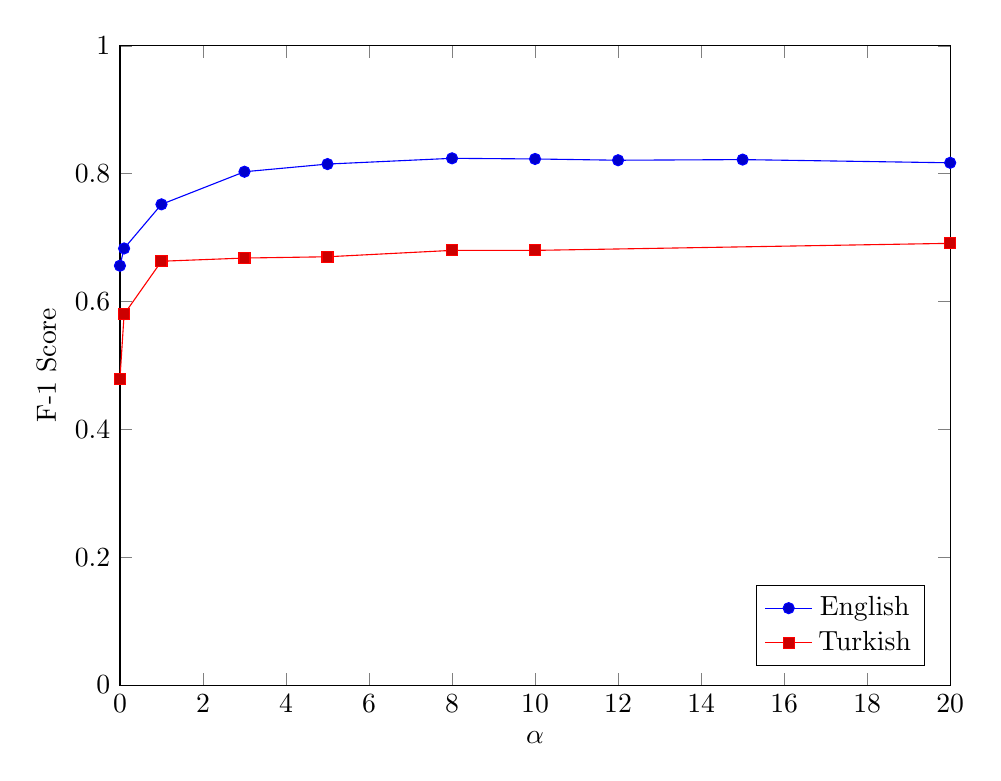
\begin{tikzpicture}
        \begin{axis}[
                height=0.8\linewidth,
                width=\linewidth,
                xmin=0, xmax=20,
                ymin=0, ymax=1,
                xlabel=$\alpha$,
                ylabel=F-1 Score,
                legend pos=south east,
            ]
            \addplot coordinates {
                (0, 0.656)
                (0.1, 0.683)
                (1, 0.752)
                (3, 0.803)
                (5, 0.815)
                (8, 0.824)
                (10, 0.823)
                (12, 0.821)
                (15, 0.822)
                (20, 0.817)
            };
            \addlegendentry{English}
            \addplot coordinates {
                (0, 0.479)
                (0.1, 0.580)
                (1, 0.663)
                (3, 0.668)
                (5, 0.670)
                (8, 0.680)
                (10, 0.680)
                (20, 0.691)
                (50, 0.697)
            };
            \addlegendentry{Turkish}
        \end{axis}
    \end{tikzpicture}
    \label{fig:supervised}
    \caption{Performance of the semi-supervised model based on $\alpha$.}
\end{figure}

We found that utilizing information from the gold segmentations, we were able to substantially increase our
performance, from an accuracy of 65.5\% to 81.7\% with English, and from 47.9\% to 69.7\% with Turkish.
This is a substantial but expected increase; observing the unsupervised model reveals that it performs
many segmentations with nonexistent affixes, which are rectified by providing input about known affixes.

It should be noted that as $\alpha$ increases, the likelihood of the labeled training data matters more and more,
and the score is positively influenced up to a point---as $\alpha$ increases further, the labeled data
dominates the loss function, and the information from the unstructured model ceases to be used,
causing a slow decline in the score.

We found that adding the additional Turkish candidates and features regarding translation
did not help accuracy of training very much; this is likely due to the incompleteness of the translation
dictionary only being able to provide potential translations for very few words. Furthermore, due to the ambiguity
of translation, it's very hard to tell whether or not something would make a good parent of a word after
translating the word into Turkish, taking the parent in Turkish, and translating it back. The additional candidates,
for the most part, reduced accuracy by increasing the number of incorrect parent choices,
as opposed to their intended result of providing parents that our candidate generation algorithms missed.
\bibliography{paper}
\bibliographystyle{plainnat}

\end{document}
